\chapter{Equations}\label{CHAP_EQ}

\footnote{This chapter corresponds to section 2 and appendix A of~\citep{velasco2019knosos}.}
In this chapter, we briefly present the equations solved by {\ttfamily KNOSOS}. Their derivation and further details can be found in previous work by~\citep{calvo2017sqrtnu,calvo2018jpp}. We first define  the coordinate system that we will use. The flux surfaces are labelled by the radial coordinate
\begin{equation}
\psi=|\Psi_t|\,,
\end{equation}
where $2\pi\Psi_t$ is the toroidal magnetic flux.  The magnetic field lines on the surface are labelled by an angular coordinate
\begin{equation}
\alpha = \theta -\iota\zeta\,,
\end{equation}
where $\theta$ and $\zeta$ are poloidal and toroidal Boozer angles, respectively, and $\iota$ is the rotational transform. Finally, $l$ is the arc-length along the magnetic field line. In these coordinates, the magnetic field $\mathbf{B}$ can be written as
\begin{eqnarray}
\mathbf{B}&=&\Psi_t'\nabla \psi \times\nabla\alpha\,,
\end{eqnarray}
where primes stand for derivatives with respect to $\psi$, and $\Psi_t'=\pm 1$ depending on whether the magnetic field is parallel or antiparallel to the direction of the Boozer toroidal angle (i.e. depending on the sign of $\mathbf{B}\cdot\nabla\zeta$).

As velocity coordinates, we choose the particle velocity
\begin{equation}
v = |\mathbf{v}|\,,
\end{equation}
the pitch-angle coordinate
\begin{equation}
\lambda=\frac{1}{B}\frac{v_\perp^2}{v^2}\,,
\end{equation}
and the sign of the parallel velocity
\begin{equation}
\sigma= \frac{v_\parallel}{|v_\parallel|}=\pm 1\,,
\end{equation}
where, as usual,
\begin{eqnarray}
v_\parallel &=& \mathbf{v}\cdot \mathbf{b} = \mathbf{v}\cdot\frac{\mathbf{B}}{|\mathbf{B}|}=  \mathbf{v}\cdot\frac{\mathbf{B}}{B}\,,\nonumber  \\
v_\perp &=& \sqrt{v^2-v_\parallel^2}\,.
\end{eqnarray}

For each species $b$ ($i$ will denote bulk ions and $e$ electrons), we need to calculate the deviation of the distribution function from a Maxwellian for trapped particles, that we denote by $g_b(\psi,\alpha,l,v,\lambda,\sigma)$. The Maxwellian distribution function reads
\begin{equation}
 F_{M,b}=n_b\left(\frac{m_b}{2\pi T_b}\right)^{3/2}\exp{\left(-\frac{m_bv^2}{2T_b}\right)}\,,
\end{equation}
where $n_b$ is the density, $T_b$ the temperature and $m_b$ the mass. Trapped particles are those for which $v_\parallel=0$ at some point along their trajectories. For them, $1/B_{max}\le\lambda\le1/B_{min}$, where $B_{max}$ and $B_{min}$ are the maximum and minimum values of the magnetic field strength on the flux surface, respectively.

The equation for $g_b(\psi,\alpha,v,\lambda)$ is
\begin{equation}
\int_{l_{b_1}}^{l_{b_2}} \frac{\mathrm{d}l}{|v_\parallel|} \mathbf{v}_{D,b}\cdot\nabla\alpha~\partial_\alpha g_b+\int_{l_{b_1}}^{l_{b_2}} \frac{\mathrm{d}l}{|v_\parallel|} \mathbf{v}_{D,b}\cdot\nabla \psi \Upsilon_b F_{M,b} =\int_{l_{b_1}}^{l_{b_2}} \frac{\mathrm{d}l}{|v_\parallel|} C_b^{\mathrm{lin}}[g_b]\,,
\label{EQ_DKEFINAL}
\end{equation}
complemented with the condition at the boundary between passing and trapped, $\lambda = 1/B_{max}$ ($B_{max}$ is the maximum value of the magnetic field strength on the flux surface),\begin{equation}
g_b (\lambda=1/B_{max})=0\,,
\label{EQ_CONT2}
\end{equation}
and the condition
\begin{equation}
\int_0^{2\pi}g_b~\mathrm{d}\alpha =0\,.
\label{EQ_CONT1}
\end{equation}
The coefficients of equation (\ref{EQ_DKEFINAL}) are integrals over the arc-length between the bounce points $l_{b_1}$ and $l_{b_2}$, i.e., between the points where the parallel velocity of the particle is zero (see a sketch in figure~\ref{FIG_ORBIT}). On the right-hand side of equation~(\ref{EQ_DKEFINAL}), $C_b^{\mathrm{lin}}[g_b]$ is the linearized pitch-angle-scattering collision operator:
\begin{equation}
C_b^{\mathrm{lin}}[g_b]=
\frac{\nu_{\lambda,b} v_{||}}{v^2 B}\partial_\lambda\left(v_{||}\lambda\partial_\lambda g_b \right)\,.
\label{EQ_COLOP}
\end{equation}
For the ions, since $\sqrt{m_e/m_i}\ll 1$, this single-species collision operator is correct, but electron-ion collisions need to be retained in the electron drift-kinetic equation. For both species, we follow the common practice (see e.g.~\citep{beidler2011icnts}) of using equation (\ref{EQ_COLOP}) with an effective collision frequency accounting for inter-species collisions, given by the sum\footnote{We note that $\nu_{\lambda,b}=2\nu_b$, with the definition of $\nu_b$ of page 3 of~\cite{beidler2011icnts}.}
\begin{equation}
\nu_{\lambda,b}=\sum_{b'}\nu_0^{b/b'}\left[\mbox{erf} \left(\sqrt{m_{b'} v^2 /(2T_{b'})}\right) - \chi \left(\sqrt{m_{b'} v^2 /(2T_{b'})} \right)\right]\,,
\end{equation}
with
\begin{equation}
\nu_0^{b/b'}= \frac{8\pi  n_{b'} {Z_b}^2{Z_{b'}}^2  e^4 \ln \Lambda^{b/b'}}{m_b^2 v^3} \,.
\end{equation}
Here, $\ln \Lambda^{b/b'}$ is the Coulomb logarithm, 
\begin{equation}
\chi (x) = \frac{\mbox{erf} (x) - (2 x/\sqrt{\pi})\exp(-x^2)}{2x^2}\,,
\end{equation}
and
\begin{equation}
\mbox{erf}(x) = \frac{2}{\sqrt{\pi}} \int_0^x \exp (- t^2)\, \mathrm{d} t
\end{equation}
is the error function.

%This is discussed in more detail in section~\ref{SEQ_COLOP}.
On the left-hand-side of equation~(\ref{EQ_DKEFINAL}), 
\begin{equation}
\Upsilon_b = \frac{\partial_\psi n_b}{n_b} + \frac{\partial_\psi T_b}{T_b}\left(\frac{m_bv^2}{2T_b}-\frac{3}{2}\right)+\frac{Z_be\partial_\psi\varphi_0}{T_b}
\end{equation}
is a combination of thermodynamical forces ($Z_b$ the charge number, and the elementary charge is denoted by $e$) and the drift velocity,
\begin{equation}
\mathbf{v}_{D,b} = \mathbf{v}_{M,b}+\mathbf{v}_E\,,
\end{equation}
is the sum of the (low $\beta$) magnetic drift and the $E\times B$ drift:
\begin{eqnarray}
\mathbf{v}_{M,b} &=& \frac{m_bv^2}{Z_be}\left(1-\frac{\lambda B}{2}\right)\frac{\mathbf{B}\times\nabla B}{B^3}\,,\nonumber\\
\mathbf{v}_E &=& -\frac{\nabla\varphi\times\mathbf{B}}{B^2}\,.
\end{eqnarray}
Here, $\varphi$ is the electrostatic potential, that can be split as
\begin{equation}
\varphi(\psi,\alpha,l)=\varphi_0(\psi)+\varphi_1(\psi,\alpha,l)\,,
\end{equation}
with
\begin{equation}
|\varphi_1|\ll|\varphi_0|\,,
\end{equation}
which means that $\varphi_0$ and $\varphi_1$ will be the dominant contribution to the radial and tangential components of the electric field, respectively (and in turn to the tangential and radial components of the $E\times B$ drift, respectively). The potentials $\varphi_0$ and $\varphi_1$ can be determined by solving two additional equations.

The component of the electrostatic potential that varies on the flux surface, $\varphi_1$, is obtained from the quasineutrality equation, which for a pure plasma (i.e., composed of electrons and one ion species) reads
\begin{equation}
\left(\frac{Z_i}{T_i}+\frac{1}{T_e}\right)\varphi_1 =\frac{2\pi}{en_e}\sum_b Z_b \int_0^\infty\mathrm{d} v \int_{B^{-1}_{{\rm max}}}^{B^{-1}}\mathrm{d}\lambda\frac{v^3 B}{|v_\parallel |}g_b\,.
\label{EQ_QNFINAL}
\end{equation}
The sum is done over kinetic species. Here, we have used that, in terms of our coordinates, velocity space integrals are of the form
\begin{equation}
\int\mathrm{d}^3v (...) = \pi \sum_\sigma\int_0^\infty\mathrm{d}v\,v^2\int_0^{B^{-1}}\mathrm{d}\lambda\frac{B}{\sqrt{1-\lambda B}} (...) \,,
\label{EQ_VELINT}
\end{equation}
that $g_b$ is even in $\sigma$ and that $g_b=0$ for $\lambda<B_{max}^{-1}$. We note that, since $\varphi_1$ and $g_b$ appear in equations (\ref{EQ_DKEFINAL}) and (\ref{EQ_QNFINAL}), both equations need to be solved consistently.

The radial electric field is given by the radial derivative of the piece of the electrostatic potential that is constant on the flux surface, 
\begin{equation}
E_r =-\partial_r\varphi_0\, = -\frac{\partial \psi}{\partial r}\partial_\psi\varphi_0\,,
\end{equation}
where $r=a\sqrt{\psi/\psi_{LCFS}}$, $\psi_{LCFS}$ being the flux-label at the last closed flux surface and $a$ the minor radius of the device. The radial electric field is set by the ambipolarity of the neoclassical radial particle fluxes,
\begin{equation}
\sum_b Z_b\Gamma_b(\partial_\psi\varphi_0) =0\,.\label{EQ_AMB}
\end{equation}
In our variables,
\begin{equation}
\Gamma_b\equiv\fsa{\pmb{\Gamma}_b\cdot\nabla r} = 2\frac{\partial r}{\partial\psi}\left\langle\int_0^\infty\mathrm{d} v \int_{B^{-1}_{{\rm max}}}^{B^{-1}}\mathrm{d}\lambda\frac{v^2 B}{\sqrt{1-\lambda B}} g_b ~\mathbf{v}_{D,b}\cdot\nabla\psi \right\rangle\nonumber\,,\label{EQ_GAMMA}
\end{equation}
where $\fsa{...}$ denotes flux-surface average. Finally, the radial energy flux is given by
\begin{equation}
Q_b\equiv\fsa{\mathbf{Q}_b\cdot\nabla r} = 2\frac{\partial r}{\partial\psi}\left\langle \int_0^\infty\mathrm{d} v \int_{B^{-1}_{{\rm max}}}^{B^{-1}}\mathrm{d}\lambda\frac{v^3 B}{\sqrt{1-\lambda B}} g_b\frac{m_bv^2}{2}\mathbf{v}_{D,b}\cdot\nabla\psi\right\rangle \,.\label{EQ_GAMMAQ}
\end{equation}

\begin{figure}
\centering
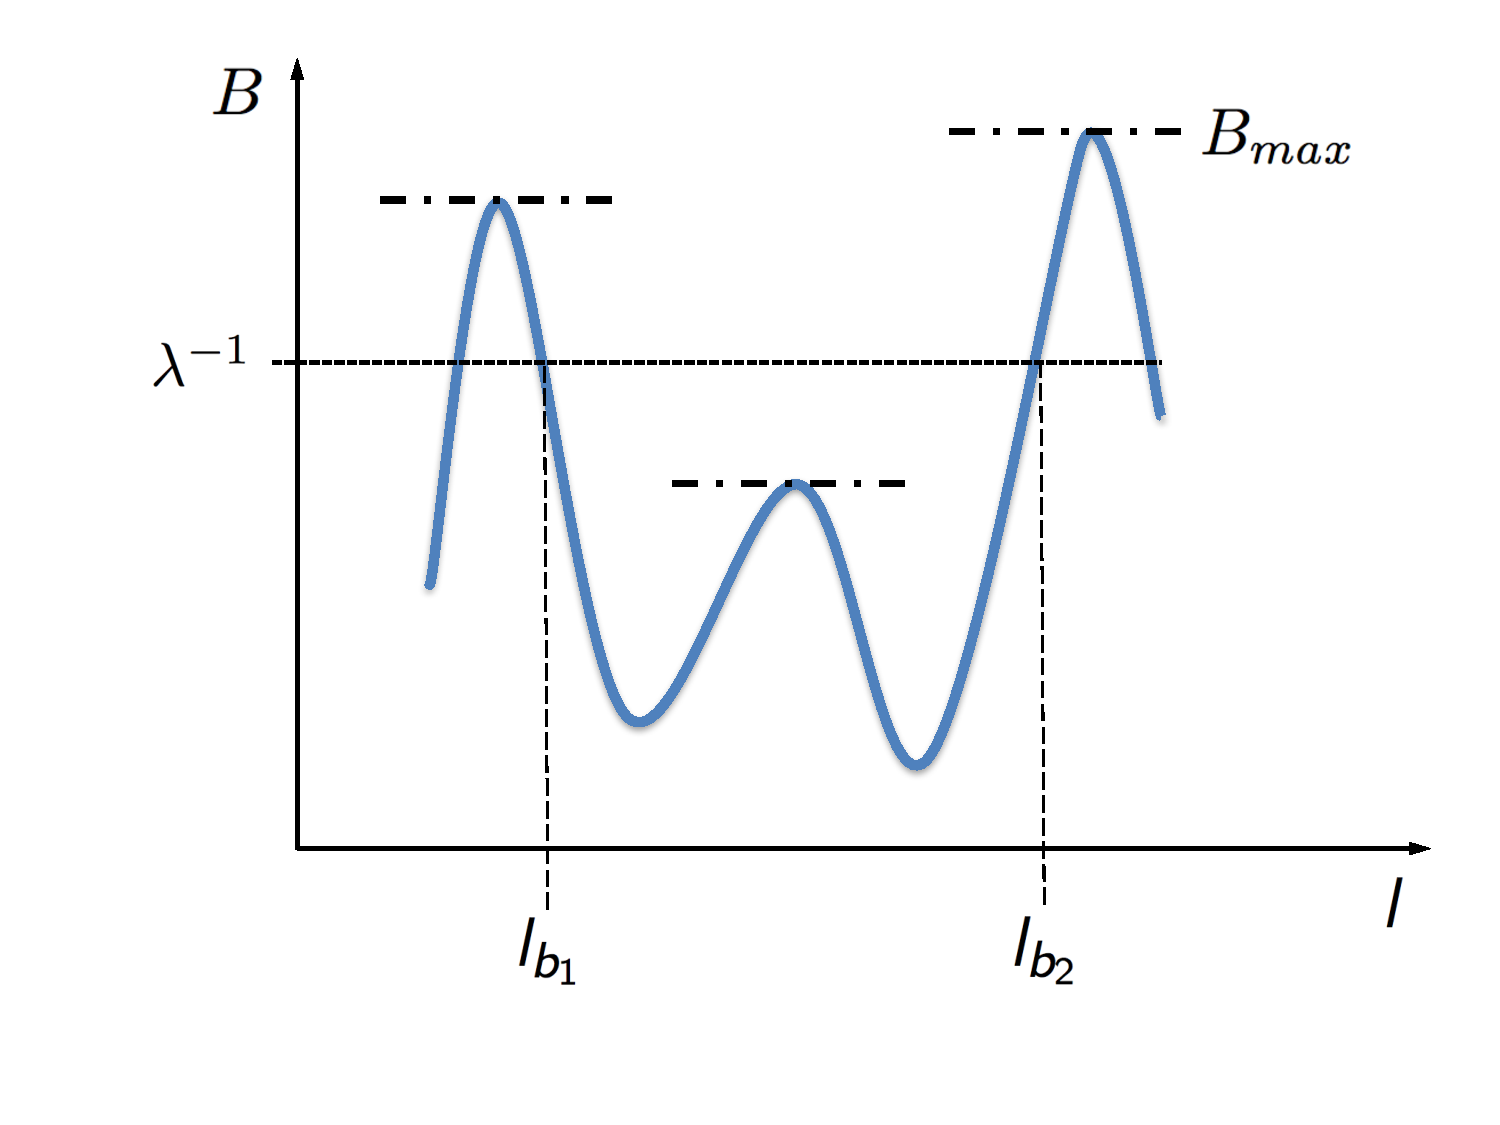
\includegraphics[angle=0,width=0.6\columnwidth]{figures/B_l}
\caption{Sketch of a particle trajectory at fixed $\alpha$. divergences are indicated with dot-dashed horizontal lines.}
\label{FIG_ORBIT}
\end{figure}

\KNOSOS~solves equations~(\ref{EQ_DKEFINAL}) and (\ref{EQ_QNFINAL}), together with equation~(\ref{EQ_AMB}). These equations have been rigorously derived in~\citep{calvo2018jpp} under the hypotheses of low collisionality, large aspect ratio and closeness to omnigeneity (we note that large aspect-ratio is a common characteristic of real stellarators~\citep{beidler2011icnts} while, as noted in the introduction, closeness to omnigeneity is a property sought in present and future devices). At low collisionalities, the motion of particles along the magnetic field is much faster than collisions, and the distribution function does not depend on the arc length $l$. Closeness to omnigeneity makes neoclassical transport describable by a radially-local equation for the deviation of the distribution function of trapped particles from a Maxwellian. In particular, it guarantees that the bounce-averaged radial drift is small enough so that
\begin{equation}
\left|\int_{l_{b_1}}^{l_{b_2}} \frac{\mathrm{d}l}{|v_\parallel|} \mathbf{v}_{D,b}\cdot\nabla\psi~\partial_\psi g_b\right|\ll
\left|\int_{l_{b_1}}^{l_{b_2}} \frac{\mathrm{d}l}{|v_\parallel|} \mathbf{v}_{D,b}\cdot\nabla\alpha~\partial_\alpha g_b\right|\,
\label{EQ_LOCAL}
\end{equation}
even in situations of small $E\times B$ drift. Hence, for stellarators close to omnigenity, terms proportional to $\partial_\psi g$ do not appear in equation~(\ref{EQ_DKEFINAL}). Finally, the large-aspect ratio approximation allows us to use the pitch-angle collision operator, equation~(\ref{EQ_COLOP}).
 
Let us finally discuss the neoclassical regimes that equations~(\ref{EQ_DKEFINAL}) and (\ref{EQ_QNFINAL}) can describe. The second term on the left-hand side of equation~(\ref{EQ_DKEFINAL}) includes the radial magnetic and $E\times B$ drifts caused by the inhomogeneity of the magnetic field strength and of the electrostatic potential on the flux surface, respectively. This means that equation~(\ref{EQ_DKEFINAL}) can model the $1/\nu$ regime and the transport caused by $\varphi_1$. The first term of the left-hand side includes the precession tangential to the flux surface caused by the radial variation of the electrostatic potential (i.e. the radial electric field $E_r$) and of the magnetic field strength. This implies that we can model the $\sqrt{\nu}$ and superbanana-plateau regimes. As discussed previously, radially global effects are not accounted for.






%\section{Details of the collision operator}\label{SEQ_COLOP}

%%%%%%%%%%%%%%%%%%%%%%%%%%%%%%%%%%%%%%%%%%%%%%%%%%%%%%%%%%%%%%%%%%%%%%%%%%%%%%%%%%%%%%%%%%%%%%%%%%%%%%%%%%%%%%%%%%%

%In this chapter, the pitch-angle-scattering collision operator has been employed, and its explicit expression has been provided in equation (\ref{EQ_COLOP}). As it has been discussed, this is a single-species collision operator, which is accurate for calculating ion transport, due to $\sqrt{m_e/m_i}\ll 1$. For electrons, however, electron-ion collisions need to be retained in the electron drift-kinetic equation. In order to overcome this limitation, an effective pitch-angle-scattering collsion frequency $\nu_{\lambda,b}$ is employed in order to account for inter-species collisions. This is done for both species, although its effect will be negligible for the ions.
%
%In this appendix, we provide the explicit expression of the pitch angle scattering frequency, given by the sum\footnote{We note that $\nu_{\lambda,b}=2\nu_b$, with the definition of $\nu_b$ of page 3 of~\cite{beidler2011icnts}.}
%\begin{equation}
%\nu_{\lambda,b}=\sum_{b'}\nu_0^{b/b'}\left[\mbox{erf} \left(\sqrt{m_{b'} v^2 /(2T_{b'})}\right) - \chi \left(\sqrt{m_{b'} v^2 /(2T_{b'})} \right)\right]\,,
%\end{equation}
%with
%\begin{equation}
%\nu_0^{b/b'}= \frac{8\pi  n_{b'} {Z_b}^2{Z_{b'}}^2  e^4 \ln \Lambda^{b/b'}}{m_b^2 v^3} \,.
%\end{equation}
%Here, $\ln \Lambda^{b/b'}$ is the Coulomb logarithm, 
%\begin{equation}
%\chi (x) = \frac{\mbox{erf} (x) - (2 x/\sqrt{\pi})\exp(-x^2)}{2x^2}\,,
%\end{equation}
%and
%\begin{equation}
%\mbox{erf}(x) = (2/\sqrt{\pi}) \int_0^x \exp (- t^2)\, \mathrm{d} t
%\end{equation}
%is the error function.

